\Chapter{Megvalósítás}


\Section{Részecske alapú}

Nézzük részletesebben a részecske alapú program megvalósítását. Maga a program 3 osztályból, egy ezeket összefogó javascript-ből, és egy CSS-ből meg egy HTML-ből áll. 

\Section{HTML}

 A HTML-ben a szokásos HTML elemek vannak, vagyis itt kötjük össze magát a programot, az osztályokat, a CSS-t és a javascript-et. Itt adjuk, meg hogy mekkora legyen a canvas amire a programot megvalósítjuk. Annyi érdekessége van, hogy a body elemben van egy eseménykezelő ami az onload, és azt a célt szolgálja, hogy az adott esemény csak az oldal betöltődése és megjelenése után következzen be.
Találunk itt még 2 db gombot, amivel a programhoz adhatunk poharat, illetve el is távolíthatjuk azt.
Illetve a HTML fájlban még találunk 2 darab táblázatot, ami különböző dolgok állítására szolgál. Az elsőben a részecskék sűrűségét, a gravitációt, a húzó erőt és a részecskék súlyát lehet állítani. 
A második táblázatban a pohárhoz tartozó koordinátákat, amiknek elnevezése x1,y1, x2,y2, x3,y3, x4,y4. Ezek a koordináták a következőképpen \Aref{fig:pohar} helyezkednek el.

A különböző beállításokra szolgáló dolgok a következőképpen jelennek meg a programban \Aref{fig:html}. Mindegyikhez tartozik egy alap érték, ami a programban bármikor módosítható. Illetve a sűrűség, gravitáció, húzó erő és a súly aktuális értéke a következőképpen \Aref{fig:ertekek} mindig megjelenik a képernyőn a canvason belül bal oldalon. 

\begin{figure}[h]
	\centering
	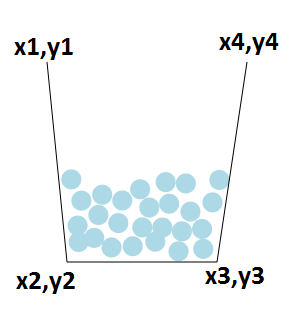
\includegraphics[scale=1]{images/pohar.png}
	\caption{Koordináták}
	\label{fig:pohar}
\end{figure}

\begin{figure}[h]
	\centering
	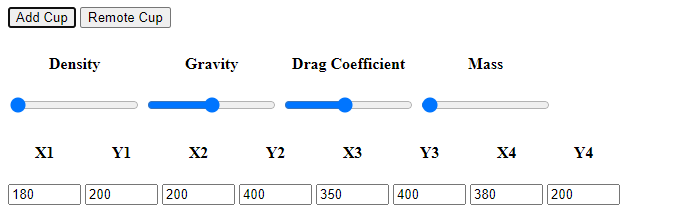
\includegraphics[scale=1]{images/html.png}
	\caption{Pohár hozzáadó/eltávolító gomb, sűrűség, gravitáció, húzó erő és súly beállító, illetve a koordináták beállítója}
	\label{fig:html}
\end{figure}

\begin{figure}[h]
	\centering
	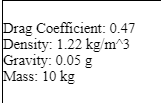
\includegraphics[scale=1]{images/ertekek.png}
	\caption{Az aktuális értékek megjelenítése}
	\label{fig:ertekek}
\end{figure}

\Section{CSS}

A CCS fájlban pedig a HTML-től is kevesebbet találunk. Egyedül a canvas-ra határozunk meg benne egy stílust, ami pedig nem más, mint hogy legyen egy 1 pixel vastagságú fekete határa/oldala.

\Section{Osztályok}

De térjünk át a program érdekesebb részeire. Először is a 3 osztályt nézzük sorban, amik a pont, részecske és a szimulátor.

\Section{Pont osztály} 

A pont osztályban még semmi érdekességet nem találhatunk, van egy constructora, getter, setter, move, eltoló és távolság számító metódus. Az utóbbit a szimulátor programban használjuk. Itt a constructor a pont x, y koordinátájára van, getter, setter pedig szinten az x, y -ra. Az eltoló metódus az x, y koordinátákhoz ad hozzá mindig egy értéket, ami a metódus hívásánál lehet átadni, hogy mennyi legyen. A távolság számító metódus pedig, ahogy a neve is mutatja távolságot számít 2 pont között. Ez a távolság számítás a matematikából is jól ismert távolságszámítás. Kivonjuk egymásból a két pont koordinátáit, majd négyzetre emeljük a kapott értékeket, azokat összeadjuk, majd pedig gyököt vonunk. 

\Section{Részecske osztály}

A részecske osztályban már több érdekességet találunk. Ez az osztály a pont leszármazottja. Neki is van construktora, getter-ek, setter-ek, és egy rajzoló metódus. Itt a construktor egy részecske tulajdonságait írja le. Minden részecskének van x,y koordinátája, színe, sebesség vektora, visszapattanási együtthatója, és mérete. Ezekben különbség a részecskék között csak az x,y koordinátákban van illetve a sebesség vektorban. A többi dolog az összes részecskére nézve azonos. Getter, setter metódusai a sugárnak és a színnek vannak. A rajzoló metódus, pedig egyetlen részecskét rajzol ki. Ez a következőképpen néz ki, a részecske színe a constructorban megadott szín lesz. Majd a koordinátája ugyaninnen az x és y koordináta , illetve a sugara is a fent megadott sugár lesz. 

\Section{Szimulátor osztály}

A szimulátor osztály a legérdekesebb, itt találhatóak a program fő részei. Itt hozzuk létre a részecskéket, rajzoljuk ki őket, itt vizsgáljuk az ütközéseket (falra, részecskék között, pohárral), itt hozzuk létre a poharat. 

\textbf{Constructor}
Először itt is van constructor, ahol azt adhatjuk meg, hogy hány db részecske legyen a programban. Ez úgy történik, hogy meghívjuk a részecskelétrehozó függvényt és paraméterként átadjuk a részecskék számát.

\textbf{Frissítés}

Van egy frissítés, ahol azt adjuk meg, hogy frissítés alkalmával mi történjen. Töröljük a canvast, majd beállítjuk a részecskék sebességét, és sebesség koordinátáit. Ez a következőképpen működik: kiszámítjuk az aerodinamikai erőket x-re is és y-ra is ezzel a képlettel $[-0.5 * Cd * A * v^2 * rho]$, az ebben a képletben szereplő Cd és A, a húzóerő és a sűrűség, ezek alap értéke 0.47 és 1.22, de ez módosítható a húzóerő 0 és 1 között, a sűrűség pedig 0 és 1000 között, majd megvizsgáljuk ezen értékeket, hogy számok-e ha számok akkor a kiszámolt értékekkel számolunk, ha nem akkor pedig 0-val. Kiszámítjuk a részecske sebesség vektorát, mivel nekünk y irányban mozognak a részecskék a gyorsulási együtthatóval ami a földön és a programban is 9.82 m/(s*s), illetve a gravitációval számolva. A programban a gravitáció alap értéke 0.05, de ez az érték 0 és 0.1 között módosítható. De ezek mellé számításba kell vennünk a részecskék súlyát is, aminek szintén van egy alap értéke, mégpedig 10kg, de ez érték is módosítható 1 és 1000kg között. Majd a részecskék x és y koordinátáihoz hozzáadva a sebesség vektort, számolva a kép frissítés értékével és szorozva 100-al az értéket, megkapjuk, a részecskék új pozícióját.

\textbf{Részecskék létrehozása}

Ebben az osztályban hozzuk létre a részecskéket is, random generálunk x és y koordinátákat, ügyelve, hogy ezek a koordináták a canvas területén belül legyenek. A canvasunk mérete 800széles és 600 magas, vagyis x koordinátákat 10 és 780, y koordinátákat pedig 10 és 580 között generálunk. Majd itt ezekkel a koordinátákkal, megadva a sugár méretét ami 10, illetve a visszapattanás értékét ami 0.7, létrehozzuk a részecskéinket. Ezeket az adatokat pedig egy tömbben tároljuk el. 

\textbf{Részecskék kirajzolása}


Végig megyünk az előbb létrehozott tömbön, amiben meg vannak az adatok a kirajzoláshoz, majd kirajzoltatjuk a részecskéket a részecske osztály kirajzoló metódusával. 


\textbf{Fallal való ütközés}

Majd jön az ütközés vizsgálat, amit először a falakra vizsgálunk meg. A fallal való ütközést külön nézzük mind a 4 falra, majd minden esetben ütközés után átállítjuk a részecske sebességvektorát, illetve a pozícióját a megfelelő értékekre. A sebesség vektort, minden esetben ugyanúgy számítjuk, szorozzuk az adott oldalhoz tartozó sebesség vektor x, vagy y koordinátáját a visszapattanási együtthatóval. A részecskék x, y koordinátájára pedig az oldal határozza meg a számításra, amire éppen nézzük az ütközést. Jobb oldalon a canvas szélességéből kell kivonni a sugarat. Bal oldalon pedig csak a sugárral kell számolnunk. Ugyanez a helyzet a felső és az alsó oldallal is. Lent a canvas magasságából vonjuk ki a kör sugarát, fent pedig csak a sugárral számolunk.

\textbf{Részecskék közötti ütközés}

A részecskék  közötti ütközés kicsit összetettebb, itt mindig 2 részecskét vizsgálunk. Először is megnézzük, hogy a két részecske koordinátája nem-e ugyanaz, ha nem, akkor megnézzük, hogy az egyik részecske koordinátája plusz a két sugár nagyobb-e, mint a másik részecske koordinátája, illetve fordítva is megnézzük, hogy kisebb-e a koordináta, mint a másik részecske koordinátája és a két sugár összegétől. Majd, ha ezek közül a feltételek közül az egyik teljesül, vagyis a két részecske túl közel van egymáshoz, akkor kiszámoljuk a távolságot, hogy milyen közel is vannak. Ha ez a távolság kisebb, mint a két sugár összege, akkor kiszámoljuk az ütközési pont koordinátáit, megszüntetjük, hogy a részecskék elfedjék egymást, majd frissítjük a sebességet az ütközés tükrében.

\textbf{Pohár kirajzolás}

A pohár rajzoláshoz a bekért koordináták értékeivel számolunk. Maga a pohár 3 vonalból áll. 


\textbf{Pohárral való ütközés}

A pohárral való ütközésvizsgálathoz is szükségesek a bekért koordináták értékei. Egy x és egy y változóba letároljuk a részecskék x és y koordinátájához hozzáadva a sebesség vektorokat. Majd megnézzük van-e ütközés. Ez a következőképpen történik, a 3 vonalra külön-külön nézzük az ütközéseket. Van 3 darab függvény amivel ezt vizsgáljuk, mindegyik vonalra egy. Ezekben a függvényekben kiszámoljuk a vonalak hosszát, majd a vonal és a kör szorzatát számoljuk. Megkeressük a vonalakhoz közeli koordinátákat. Majd egy másik függvénnyel megvizsgáljuk, hogy a körök milyen távol vannak a vonalaktól. Ez úgy történik, hogy kiszámoljuk a pont távolságát a vonal 2 végpontjától, majd a vonalak hosszát, majd megadunk egy tűréshatárt ami itt 0.1 és megnézzük, hogy a körök távolsága a vonalak végétől, hogyan viszonyulnak a vonalak hosszához. Majd visszatérve az előző függvénybe kiszámoljuk a távolságát a közeli pontoknak, majd ha ez kisebb mint a sugár akkor igaz az ütközés. 


A részecske osztály ezeket tartalmazná. 

\textbf{Összefoglaló javascript}

Most nézzük az ezeket összefogó javascript miket tartalmaz. Ez az egész egy funkció, ami mint már említettem a HTML-ben van meghívva egy eseménykezelővel. Ebben van benne a szimulátor létrehozása, a canvas beállítása, és egy funkció a frissítésre, ami 60 fps-el frissít, és meghívja a szimulátor metódusait, a frissítést, rajzolást és ütközésvizsgálatokat. Illetve van 2 funkció, amik a pohár hozzáadásához illetve eltávolításához szükséges. Van egy pohár változó ami vagy igaz vagy hamis, annak az értékét módosítjuk itt. Majd ha igaz, akkor az előbb említett frissítésnél meghívja a pohár kirajzoló metódust, illetve az arra vonatkozó ütközésvizsgálatot.  

